\documentclass[12pt]{article}
\usepackage[a4paper, total={6in, 8in}]{geometry}
\usepackage[utf8]{inputenc}
\usepackage[round]{natbib}
\usepackage{graphicx}
\usepackage{dblfloatfix}    % To enable figures at the bottom of page
\usepackage{rotating}
\usepackage{tikz}
\usepackage{authblk}
\usepackage{booktabs, tabularx}
\usepackage{amsmath}
\usepackage[input-decimal-markers=.]{siunitx}
\usepackage[english]{babel}
\usepackage{pdflscape}
\usepackage{setspace} \doublespacing
\usepackage{dcolumn,caption}
\usepackage{array, threeparttable} % to add footnotes to the tables
\setlength{\emergencystretch}{3em}
\captionsetup{skip=0.333\baselineskip}
\newcolumntype{d}[1]{D{.}{.}{#1}}
\newcommand\mc[1]{\multicolumn{1}{@{}c@{}}{#1}} % handy shortcut macro

\begin{document}

\title{What start-up teams are funded and why: \\ empirical evidence from social proof signaling role}
\date{\vspace{-3ex}}
\author{Arnauld Bessagnet \\ \footnotesize{LEREPS – Sciences-Po Toulouse, University of Toulouse – France} \\}

\maketitle \vspace{-1,5em}

\begin{abstract}
\noindent
Entrepreneurship research and signaling theory suggests that start-up teams' human capital has a signal-quality effect on how easily they can access financial resource from investors. Based on a sample of 508 software-based firms, we examine the signal effect of skills and expertise endorsement, a peer-reviewed relational measure of professional capabilities, and its influence on the amount of external funding received in early stage. Results show that investors favor start-up teams that have either a high level of competency or a high level of variety of skills, but only some at once. We discuss the implications of these findings for the research literature on digital entrepreneurship and venture capital. \newline

\begin{obeylines}
\noindent \footnotesize{}{\textbf{Keywords:} Skills, Entrepreneurship, Fundraising, Start-up Teams, Variety}
\noindent \footnotesize{\textbf{JEL Classification:} L22, L26, L85}
\end{obeylines}

\end{abstract}

\clearpage
\section{Introduction}

%I want you to act as an academician. Read this text and rephrase it for academic readings. This new text must not be spotted by plagiarism detector.

%Ok, again, I want you to act exactly like grammarly : give me  feedback on grammar, spelling, and other writing issues on the following text please. Remember : act like a scholars.

Start-up teams, i.e. individuals who jointly create a firm and are characterized on a continuum including equity ownership, decision-making autonomy and entitativeness \citep{kamm1990entrepreneurial, knight2020start}, are considered important actors for cities, regions and countries development \citep{audretsch2001linking, autio2016entrepreneurship}. As financial resource acquisition is an important part of start-up teams growth and development \citep{rosenbusch2013does}, the determinants and mechanisms to attract such resources to survive and grow are of great interest to researchers, practitioners, and policy makers \citep{EUcommission2015digital}. This interest is particularly salient in the context of the digital economy, where low-resource-intensive (efficient, predictable, and repeatable) systems offer investors new opportunities due to the non-linear revenues of digital technologies \citep{nambisan2017digital, sahut2021age}. This article contributes to this critical agenda by examining the relationship between start-up teams' human capital signals and their performance, which we examine here from the angle of resource access, specifically the access to external capital financing from professionals investors.

This research seeks to investigate the effect of skills and expertise endorsements, i.e., a peer-reviewed relational measure of professional capabilities, on the ability of start-up teams to acquire financial resources from professional investors. Which start-up teams are funded by external investors and why are recurring themes in contemporary economic and entrepreneurial literature \citep{baum2004picking, beckman2007early, bernstein2017attracting, franke2006you, franke2008venture, plummer2016better, kaplan2009should, shane2002network}. Previous studies have largely focused on the individual qualities of founding members, such as education, work experience and prior entrepreneurial endeavors, in order to explain the acquisition of financial resources by start-up teams \citep{shane2002network, hsu2007experienced}. While these studies have yielded several important insights, this approach is problematic as, nowadays, investors draw on a wide array of other signals to assess the relevance of investing in a start-up team, such as social proof data available on social networks. As this approach has been underexplored by researchers, this study examine the effect of skills and expertise endorsements (a social proof data available on LinkedIn, the world's largest professional online social network) on resource acquisition. This feature allows users to tag themselves with topics representing their area of expertise and have their connections provide social proof of their competency in that topic.

Using data from a sample of 508 software-based ventures listed on Crunchbase, Dealroom and BPI combined with data from LinkedIn, company websites and press articles, we constructed a unique dataset which includes human capital investments (i.e., common traditional signals used by investors such as years of education, professional experience and previous founding experience) and social proof outcomes of human capital (i.e., skills and expertise endorsements) of start-up teams. We test our claim in two steps. First, we examine the relationship between the signal of the level of skills and expertise endorsement of start-up teams and its impact on capital acquisitions in early stage investment. Secondly, drawing from cognitive distance model \citep{nooteboom2007optimal} and the cybernetics principles of requisit variety \citep{ashby1957introduction}, we assess the extent to which signals from startup-teams' skills and expertise endorsements variety help the firm acquire capital. Following our claims, we find that investors favor start-up teams that have either a high level of competency or a high level of variety of skills, but only some at once.

Our study contributes to the literature on signaling and new venture financing in multiple ways. First, this study presents a new approach to examining the signaling role of the composition of start-up teams \citep{beckman2007early}. Previous research has generally focused on either the proficiency level or variety of skills possessed by start-up teams. However, neither dimension by itself is sufficient to explain the success of the firm. In addition, the digital context is subject to different social and technological factors requiring a different type of signal- quality by investors and to logics of different natures \citep{nambisan2017digital}. The proposed methodology evaluates both proficiency and variety of skills simultaneously within this digital context. Second, various empirical studies on the impact of the composition of start-up teams on investors' evaluations have been conducted, taking into consideration indicators such as founders' education \citep{franke2008venture}, entrepreneurial experience \citep{beckman2007early}, industry experience \citep{becker2015new}, or leadership experience \citep{hoenig2015quality}. This article proposes a complementary approach, focusing on the 'outcomes of human capital' (i.e. the knowledge, skills and abilities), which are considered to be more precise and direct indicators than those related to 'investment in human capital' such as education and years of experience \citep{unger2011human, marvel2016human}. Methodologycally speaking, we derive from a peer-reviewed relational measure an outcome-based human capital indicator and consider it as one approach to analyzing how skills and expertise endorsement affect firms' resource acquisition. Third, this study presents a unique dataset which combines multiple sources of validated data (including Crunchbase, Dealroom, BPI, LinkedIn, company websites and press articles). We make use of CrunchBase and LinkedIn especially, as they provide reliable self-reported information which can accurately capture an individual's human capital trajectories (see previous academic work byf or e.g.,  \citet{sako2020scaling}, \citet{rapanta2017linkedin}, or \citet{reese2020should}. Consequently, this study highlights the data limitations researchers currently face when studying the acquisition of financial resources by firms. Current datasets lack information on both founder characteristics (such as occupation and education) and attributes of small firms (employment size, financial resources). By collecting data from LinkedIn, we have constructed a dataset which covers over 508 start-up teams in France. This paper serves to demonstrate the value of the data for research, particularly to understand the dynamics of signals in entrepreneurship.

The paper is structured as follows. Section 2 reviews the literature on signaling theory for early-stage resource acquisition. Section 3 explains the data and methods used, and Section 4 presents key findings. Finally, section 5 concludes by discussing implications for theory and practice, noting the limitations of this study.

%I want you to act as an academician. Read this text and rephrase it for academic readings and must not be spotted by plagiarism detector.

\section{Theoretical framework and hypothesis}

\subsection{Signaling theory for early-stage resource acquisition}

Literature on entrepreneurship has continually underscored the critical role of external financial resources for the survival and growth of new firms \citep{cooper1994initial}. Despite the numerous types of external financial sources obtainable to start-up teams \citep{drover2017review, klein2020start}, the majority of research has concentrated on the acquisition of capital from external investors, who provide financial capital in return for a stake in the company's ownership. Nevertheless, securing external funding from external investors is a challenging task, with investors having difficulty predicting which teams will come out on top \citep{ghassemiautomated, duhigg2016google}, due to the inherent information asymmetries between entrepreneurs and investors or the lack of past financial results. In order to mitigate the information asymmetries, investors lean on quality-signals \citep{spence1978job, ko2018signaling}, with signalling theory being particularly applicable in the digital context, where new digital technologies have transformed the nature of uncertainty inherent in entrepreneurial processes \citep{nambisan2017digital}.

Signaling theory posits that two parties take conscious and voluntary steps to reduce asymmetric information and perceived uncertainty between them, and this is done by focusing on the signals available to them \citep{spence1974market}. This concept has been used in various disciplines to provide insight into social selection problems when there is an absence of perfect information \citep{connelly2011signaling, colombo2021use}. Entrepreneurship scholars have found this concept to be beneficial as particular signals can diminish uncertainty about ventures' quality in the eyes of stakeholders, such as prestigious government grants \citep{islam2018signaling}, the enthusiasm and passion of the founders \citep{chen2009entrepreneur}, affiliations of the venture with other entities \citep{plummer2016better}, and the composition of the founders' team \citep{ko2018signaling}. Investors, similarly, use a variety of indicators to mitigate asymmetric information such as the founders' ties to others \citep{shane2002network}, their human capital \citep{beckman2007early}, social capital \citep{shane2002organizational}, and endorsements \citep{courtney2017resolving, janney2006moderating, plummer2016better}.

In the context of early-stage ventures, human capital of the start-up teams is considered to be a significant and prominent factor for investors to consider \citep{beckman2007early, ko2018signaling, matusik2008values}. This emphasis is due to the limited resources and small number of people responsible for formulating and carrying out strategies. According to the organizational theory perspectove applied to the entrepreneurship field, the human capital composition of the start-up teams is believed to have an imprinting effect on the processes and operations of the firm \citep{packalen2007complementing}. This concept implies that past experiences, and therefore the underlying skills and experiences acquired meanwhile, can shape the present performance. Concretely, investors aim to reduce uncertainty about the quality of the firm by relying on the human capital and demographic characteristics of start-up teams such as their educational background or their functional skills because these are easily accessible quality-signals \citep{colombo2005founders, beckman2007early, eddleston2016you, plummer2016better}.

Extensive research has been conducted to explore the association between signaling and the acquisition of financial resources (see \citep{connelly2011signaling} and \citet{colombo2021use} for a review). However, few studies have examined the connection between signals of "social proof data" available on social networks and financial resource acquisition in the early stages of venture creation. This gap in the literature is remarkable given that the level of uncertainty \citep{matusik2008values} and information asymmetry between the signal sender and receiver \citep{spence2002signaling} are most pronounced during this period. Therefore, any kind of quality-signals that help gain additional perspective and triangulate start-up teams data is welcomed by investors. At this juncture, a new venture typically has no track record of performance to rely on, yet must still find a way to convince stakeholders that it is a legitimate venture \citep{becker2015new}, and thus worthy of obtaining necessary resources, such as financial capital \citep{ko2018signaling}.

This paper proposes to investigate how investors rely on "social proof data" signals to determine the potential of new firms they are considering investing in. To this end, we will focus on the signal effect of skills and expertise endorsement, a peer-reviewed relational measure of professional capabilities feature on LinkedIn, the world's largest professional online social network. This feature enables members to tag themselves with topics representing their areas of expertise and their connections to provide social proof via the endorsement of said member's competency in the topic. From a methodological point of view, we derived an outcome-based human capital indicator based on skills and expertise endorsement data which is considered a more direct measure of human capital and as one way of analyzing how skills affect firms' performance in a digital environment \citep{marvel2016human}.

\subsection{Signaling effects from start-up teams' level of skills and expertise endorsement}

Entrepreneurship researchers have extensively explored what start-up teams' characteristics enable them to access external funding \citep{roure1990predictors}. The focus on start-up teams stems from the fact that most entrepreneurial initiatives are run mainly by groups of individuals rather than by lone individuals \citep{klotz2014new}. Such characteristics include the teams' social capital \citep{shane2002network}, the team's demographics and size \citep{eisenhardt1990organizational}, the industry environment \citep{townsend2015turning}, the teams' match with an investor's characteristics \citep{aggarwal2015evaluating} or the investor's experience \citep{franke2008venture}. However, in the context of early-stage ventures, human capital of the start-up teams is maybe the most significant and prominent factor for investors to consider \citep{beckman2007early, ko2018signaling, matusik2008values}.

The entrepreneurship literature flexibly defines human capital and includes individuals' knowledge and skills \citep{becker1964human, marvel2016human}. In this this study, conformed to the human capital literature applied to the entrepreneurial field, we postulate that start-up teams with higher levels of skills have a greater propensity to reach specific entrepreneurial milestones, elicit greater investor confidence, and a greater likelihood of attracting external financial capital. Indeed, it has been shown that higher levels of skills enable founders to take greater risks and demonstrate proactive behavior \citep{becherer1999proactive}, allowing them to optimize business opportunities \citep{shane2000promise, chandler1994founder}. Additionally, the acquired skills enable entrepreneurs to make full use of the available technological tools in a digital context \citep{nambisan2017digital}, enabling them to better understand and differentiate their offerings through the introduction of new technologies and disruptive products \citep{marvel2007technology}. Moreover, a high level of skill proficiency can help entreprneurs to obtain resources complementary to financial resources, which is an issue for many firms in the early stages of development \citep{beckman2007early, zarutskie2010role}. Finally, developing skills and knowledge is a prerequisite for further entrepreneurial learning and helps business owners acquire additional skills and knowledge that will help their firm grow \citep{hunter1986cognitive}.

Therefore, for all these reasons, we propose that a high level of skills and expertise endorsements within a start-up team enhances the quality of the signal intended for investors looking to engage financially in the early stages. The investors are alterted by this signal because it suggests that higher skill levels may translate into future success, which should draw early-stage investors. Thus, we hypothesize the following: \\

\noindent \textit{H1: Start-up teams with greater skills and expertise endorsement levels will get more fundings from investors}

\subsection{Signaling effects from start-up teams' variety of skills and expertise endorsement}

In this study, we consider not only the level of skills but also their variety \citep{harrison2007s, grillitsch2021does}. Skills' variety in a start-up team matters because the success of entrepreneurial initiatives is often the result of teamwork and collective endeavors, which require the combination of knowledge, the synergy of abilities, and the collaboration of multiple individuals \citep{klotz2014new}. This paper argue that start-up teams with a wide range of skills and expertise endorsement have a greater chance of acquiring investors due to two key reasons.

The first reason relates to the decision-making process. The underlying argument is that groups with various skills take better decisions because they have access to more information \citep{hong2001problem}. Therefore, the solutions to new issues encountered during entrepreneurial cycles might result from recombining existing knowledge under new forms. A meta-analysis conducted by \citet{jin2017entrepreneurial} suggests that an entrepreneurial teams endowed with a varied skill set are more likely to use various market entry, internationalization or innovation strategies \citep{boeker1989strategic}. This implies that start-up teams with diverse skills are in a better position to make high-quality decisions, thus increasing their chances of success. Consequently, investors may use start-up teams' skills diversity as a signal to assess their future performance, which can significantly impact the probability of receiving investments.

The second reason related to the connection between start-up teams' skills and expertise diversity and their social capital. The literature demonstrates that the social capital of a start-up team has the capacity to act as control for information asymmetries. Indeed, \citet{huang2017resources, shane2002organizational} posit that the presence of a social connection between start-up teams and investors can reduce the informational gap between them. Specifically, \citet{shane2002network} infer that social capital play a role in connecting start-up teams to potential investors and facilitating fundraising. Additionally, \citet{hoenig2015quality} suggest that the social capital of a start-up team is utilized by investors to triangulate the quality of the firm and the composition of start-up teams and their relationships are used as indicators of quality by investors \citep{plummer2016better, semrau2014exactly}. Following these rationales, if a start-up team's diversity of skills is the result of different social capital and given that capital influences the start-up teams' ability to raise funds from investors, start-up teams with diverse skill might therefore raise more funds than less diversed ones. Thus, we hypothesize the following: \\

\noindent \textit{H2: Start-up teams with greater skills and expertise endorsement variety will get more fundings from investors} \\

Following the past two rationales invite us to think that having high both highly skilled individuals and a high levels of variety within a startup team is beneficial for firm performance. However past findings suggest that adding more human capital to a start-up team does not necessarily translate into greater success \citep{pierce2013too}.

Indeed, if empirical studies suggest that a certain level of human capital stimulates the discovery of new business opportunities \citep{shane2000promise, marvel2016human}, increases the likelihood of developing radically new and commercially viable products \citep{marvel2007technology}, and increases the odds of securing external funding \citep{beckman2007early}, findings of cognitive and social psychology indicate that highly skilled individuals tend to have higher cognitive rigidity. This can be attributed to the fact that long-term exposure to a specific discipline leads to a mentality where solutions and situations are addressed according to the dominant logic paradigm of the discipline. While this cognitive rigidity can lead to greater determination, better products, and improved ability to recognize and take advantage of business opportunities.

The perils of cognitive rigidity are both more likely and especially threatening when two or more individuals also have high cognitive distance. Cognitive distance reflects the extent to which two individuals have developed different mental models, belief systems, vocabularies, and priorities \citep{nooteboom2007optimal}. Cognitive distance can impede interaction and communication with other start-up team members and make people less likely to be open to radically different logic, such as pivoting and successfully executing new business alternatives \citep{kirtley2020pivot}. While any two people are always cognitive distant to some extent, individuals who share the same skills and expertises tend to have lower cognitive distance because they are more likely to be familiar with each other’s mental models, and to build the mutual trust that is necessary for the effective functioning of a social group. Conversely, individuals who are endowed with completely different skills and expertises are less likely to have similar worldviews, knowledge, which increases their cognitive distance. In turn, this reduces the quality of both their interactions and their decisions, and the ability to interact effectively. Since the negative effects of cognitive distance are more extreme when group members have crystallized mental models and are entrenched in their opinions and positions (i.e., when they are cognitively rigid), start-up teams memebrs who are highly skilled in different disciplines are less likely to take advantage of the benefits of their broader skill sets, information, and social capital endowments. Thus, we hypothesize the following: \\

\noindent \textit{H3: Start-up teams' skill and expertise endorsement variety impact negatively the positive effect of level of skill and expertise endorsement on the funds raised} \\

Our formal hypotheses (H1, H2, H3) conform with the proposed model presented in Figure \ref{Figure1}

\begin{figure*}[!b]
  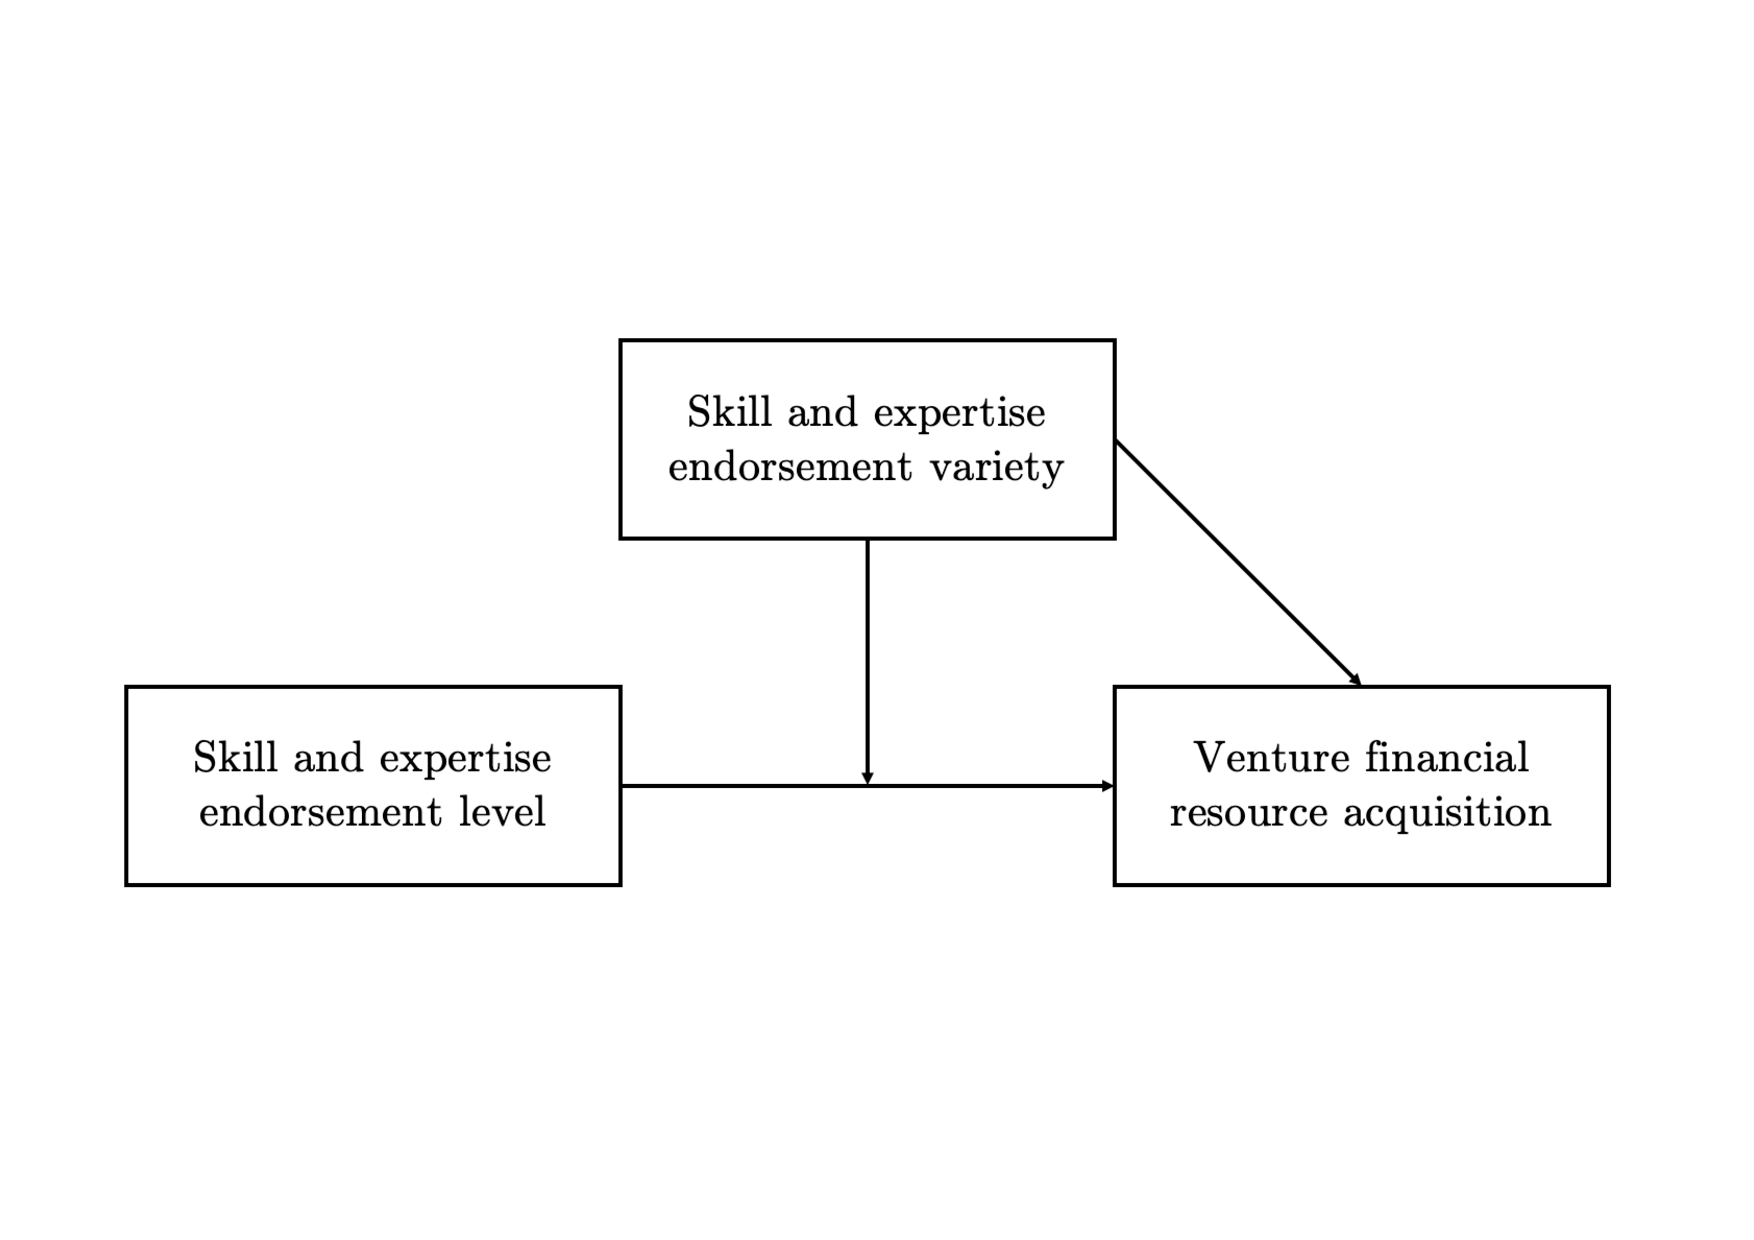
\includegraphics[width=\linewidth, scale=0.5]{model.pdf}
  \caption{Research Model}
  \label{Figure1}
\end{figure*}

\section{Methodology}

\subsection{Data sources and collection process}

To test our hypotheses, we built a dataset with information on firms, their fundraising activities, and granular information on the skill and expertises of start-up teams' members. Table \label{table1} lists our empirical variables, definitions, and sources. Table \label{table2} provides the general statistics and distribution across sizes and sectors. Table TABLE3 provides the descriptive statistics of the fundraising activities of the 508 firms in our sample. We detail the collection process below. \\

INSERT TABLE 1 HERE \\

First, we draw on Crunchbase, Dealroom, and BPI databases as a starting point. These databases provide information on the firm's headquarters, founders' names, fundraising activity, business models, and date foundation. We collected this data in March 2020 and kept firms that (i) were founded between 2010 and 2018, (ii) had their headquarters in the Metropolis of Greater Paris (France), (iii) were independent (no subsidiaries), (iv) operate in business to business markets and (v) used digital Software-as-a-Service (SaaS) business models. From these filters, we ended up with 498 SaaS digital firms\footnote{Regarding the filters (iv) and (v), we manually checked each firm's websites to check if their offers included hardware devices and if they depended on a parent company. These filters eliminated x firms (x firms with hardware business propositions and x subsidiaries)}. These criteria were chosen as a way to pinpoint the mechanisms that matter most to start-up teams working a given context. In fact, the dynamics of composition for start-up teams based in other regions may differ significantly; sampling start-up teams from a broad landscape could introduce noise into a focused investigation. Therefore, we could create accurate theoretical models for one particular area (Metropolis of Greater Paris) and domain (the digital) through focused research, in order to produce practical guidance for start-up teams' leaders and members in that location\footnote{We chose to study SaaS-based digital firms because their scalability echoes the efficient, predictable, and repeatable systems that provide investors with new opportunities offered by the non-linear revenues of digital technologies (the hardware being complicated to finance by investors) \citep{nambisan2017digital}. Also, we chose the period 2010-2018 because it fits with private firms' mass adoption of cloud technologies in pre-existing markets. Indeed, these technologies recently revolutionized the software industry in various markets, e.g., supply chain, financial, accounting, human resources, or customer relationships, making it a topic of interest in various industries \citep{luoma2018exploring}. Furthermore, we chose the Metropolis of Greater Paris (France) because it is a significant global city with labor and financial capital pools and proximate clients. The Metropolis of Greater Paris' financing and business landscape, especially its venture capital market, is one of Europe's largest, most structured, and most dynamic. From 2016 to 2020, SaaS-based firms accounted for 50\% of the total amount raised in France, 75\% of French fundraising rounds in Paris, and more than 85\% of the amount and in values (BPI, 2020)}. \\

INSERT TABLES 2 AND 3 HERE \\

Secondly, we use LinkedIn, a social networking service providing information on individuals' professional trajectories, to collect human capital - skills data of entrepreneurial teams of 498 digital firms, representing a total of x individuals. Virtual skill endorsement (skills endorsed and validated by peers on LinkedIn) is a socially constructed online reputation considered a piece of valuable information. Skill endorsement a way of self-presentation through which the job seekers brand themselves to the potential recruiters \citep{rapanta2017linkedin}. Using Linkedin has proven its relevance in recent entrepreneurship studies because it profiles detailed individual-level human capital data not available through more traditional sources. We selected carefully all founders that possess equity in the firm \citep{knight2020start, xie2020does}. Table TABLE4 list the descriptives statistics of all variables (means, std dev, min, max). \\

INSERT TABLE 4 HERE

\subsection{Dependent variable: fundraising}

La performance des firmes digitales a été opérationnalisée de nombreuses façons parce qu'il n'y a pas de consensus dans la littérature sur la façon de mesurer leur performance. Par exemple, les chercheurs ont opérationnalisé la performance en termes de croissance (des ventes, d'emplois, de revenus), de rentabilité, de survie, d'innovation ou d'introduction en bourse (IPO) \citep{delmar2003arriving}.

L'obtention d'un financement externe par un investisseur est la façon dont nous évaluons la performance des firmes digitales. Nous avons choisi la métrique \textit{fundraising} car des recherches antérieures indiquent que recevoir un financement d'un investisseur est un prédicteur important de la survie et de la croissance future d'une firme \citep{beckman2007early}. Notamment, l'insuffisance des ressources financières est fréquemment citée comme la principale cause de l'échec des nouvelles entreprises au début de leur cycle de vie \citep{franke2008venture, eddleston2016you}. Nous avons donc deux populations bien distinctes dans notre échantillon : les firmes ayant reçu un financement de la part d'investisseurs externes, et celles n'en ayant pas reçu. Conformément aux études précédentes, nous utilisons le logarithme du premier tour de financement (\textit{log fundraising}). Cette variable s'étend de x à une valeur maximale de x.

Enfin, nous avons ajouté la variable (\textit{time to fundraising}) car du point de vue d'une start-up team, il est souhaitable d'obtenir un financement externe, idéalement peu de temps après la création de l'entreprise, afin d'embaucher plus de personnel et de faire croître l'entreprise. Nous utilisons Crunchbase pour identifier la date de création de l'entreprise et la date à laquelle le premier financement externe a été annoncé. Cette variable s'étend de x à une valeur maximale de x.

\subsection{Independant variables}

Le niveau de compétences est mesuré au travers d'une variable continue que nous nommons \textit{level skills}, allant de x à x (x = faible niveau de compétences ; x = niveau maximum de compétences). Tous les individus sont placés sur ce continuum dans chacun des cluster de compétence que nous avons récupéré de Linkedin. Nous attribuons à chaque start-ups teams de notre échantillon le score le plus élevé associé à l'un de ses fondateurs. Nous avons construit cette variable comme une variable continue car nous soutenons qu'un clustering dur (catégories) ne rendrait pas compte de la versatilité de l'effet proportionnel qu'il pourrait avoir sur la collecte de fonds (fuzzy clustering). Par conséquent, un score élevé correspond à un avantage supplémentaire pour les start-ups teams.

La variété des compétences est mesuré au travers d'une variable continue que nous nommons \textit{variety skills}, allant de x à x (x = faible variété de compétences ; x = maximum variété compétences). Une start-ups team est considérée comme plus variée sur le plan fonctionnel si les individus sont également répartis dans toutes les différentes catégories fonctionnelles (Blau, 1977 / Hirshman), qui sont des groupes ayant des backgrounds communs. Following \citet{harrison2007s}, we interpret a \textit{variety skills} as \textit{the composition of differences in skills among agents of a unit member}, being here the start-up team. Based on Linkedin individuals' skills and competencies data (from 1,100 unique agents, we gather 10,638 skills, including 5,449 unique skills). We assigned each founders in the dataset a score in ten functional areas (strategy, marketing, entrepreneurship, sales, software development, product, finance, management, human resources, and design). We used a bottom-up hierarchical clustering approach with Kruskal's minimum spanning tree algorithm \citep{kruskal1956shortest} and considered the occurrences and co-occurrences of skills between founders. Therefore, the similarity between any pair of skills is naturally defined as the “intersection over union”. Consequently, we set a founders' affinity to any skill cluster in the tree by measuring the skills they share. Instead of assigning a founder to the cluster with the highest affinity (hard clustering) that would not account for its versatility, we describe a founder with his set of affinities to the skills of interest (fuzzy clustering). Finally, we aggregated the founders's variety scores at the start-up team level. We can follow Mintzberg et Waters (1982), Pavett et Lou (1983) et Shein (1987) : il existe 3 rôles dans les entreprises : entrepreneurial (sales SaaS, Biz strat, designer, creation), manager (HR, finance, lawyer) et techniques (utilisation d'outils, procédures, techniques).

\subsection{Control variables}

We have ve included several control variables because the influence of other factors could skew our estimation.

First, we used the variable \textit{size} to control for start-up team's numerosity. Indeed a higher skill level and a greater variety of skills and conflicts among the members of an organization are implied by a larger population of individuals \citep{eisenhardt1990organizational}. Our sample has groups ranging in size from x to x.

Secondly, we used the variable \textit{previous founder} whose minimum and maximum values are x and x, respectively, to control the number of firms previously founded by the individuals in our sample. Indeed, a more extensive entrepreneurial experience can increase investor confidence, send a signal of competence, and have an impact on the amount of raised funds. Prior successful foundational experience — mainly financial — increases the likelihood of financing and firm valuation \citep{hsu2007experienced}.

Thirdly, using the variable \textit{previous fundraising}, we controlled whether members of the start-up team had previously raised money from investors. Though the investors believe it, it is exceedingly difficult to determine whether serial entrepreneurs are better or worse than the other founders. Even serial entrepreneurs who have failed receive much better terms from investors even though their businesses perform less well when they receive funding \citep{nahata2019success}.

With the variable \textit{previous exit}, we partially controlled whether members of the start-up team had previously completed a successful exit. Indeed, \citet{gompers2010performance} suggests founders who start successful firms have much higher success rates in subsequent firms than founders of unsuccessful firms or first-time founders.

Also, with the \textit{previous career} control variable, we could determine whether the start-up team members had any significant prior professional experience. Indeed, using human capital and signaling theory,  \citet{subramanian2022backing} investigated whether and how the human capital indicators of founders' educational attainment, professional experience, and personality traits affect early-stage venture capital (VC) investment. They concluded that founders with extensive professional experience attract higher initial investments than other founders.

Sixth, we used the \textit{previous education} variable to determine whether the members of a start-up team attended a prestigious university. Indeed, X demonstrated that founders with degrees from first-plan institutions attracted significant early-stage investments. Additionally, teams founded by Ph.D. holders are more likely to receive funding and higher valuations, suggesting a signal effect. We Therefore have added the \textit{previous Ph.D.} variable \citep{hsu2007experienced}.

Finally, we controlled for the birth date and industry in which the firm operates because there may be some confusion due to the financial circumstances in which digital firms operate. We have created six sectoral economic indicators (RH, BI), and one for each year between 2010 and 2018.

To add : \citet{ratzinger2018impact}

\subsection{Econometric Specification}

Dans cette étude, nous utilisons un Modèle linéaire généralisé utilisant une distribution binomiale négative. La régression binomiale négative sert à modéliser les variables de comptage, généralement pour les variables de résultat de comptage surdispersées (ici, le montant levé par la firme digitale) https://stats.oarc.ucla.edu/r/dae/negative-binomial-regression/

\section{Results}

\subsection{Findings}


\subsection{Robustness tests}


\section{Discussion}

Which start-up teams are funded by external investors and why are recurring themes in contemporary economic and entrepreneurial literature \citep{baum2004picking, beckman2007early, bernstein2017attracting, franke2006you, franke2008venture, plummer2016better, kaplan2009should, shane2002network}.

According to the literature, there are two types of diversity: surface-level differences (e.g., race, ethnic origin, age, etc.), and deep differences (e.g., education, skills, capacities, attitudes and personalities) \citep{bell2007deep}.

This article investigates how start-up teams' compositions affect investors' assessments. By highlighting the significance of start-up teams' skill level and skill diversity in obtaining private funding, we try to understand why the results of previous studies on start-up teams' human capital could have been more consistent. Indeed, empiric results from entrepreneurship research have highlighted the founders' human capital as the primary driver of their ability to expand. However, these studies needed did not demonstrate how the skill level and skill diversity within a start-up team can influence a digital firm's success. By examining these two metrics together, this article attempts to center the investigation on the dynamics of early-stage start-up teams and determine how vital these characteristics are to the dynamics of interactions among team members and how they relate to the structure's proper operation. Given the significance of digital firms as a catalyst for economic development, these perspectives are significant for researchers, entrepreneurs, and policymakers.

The lack of research on multiple levels regarding human capital is the primary motivation behind this study. One issue is that the results of \citep{marvel2016human} show a strong bias toward the individual level, with little consideration given to the founding team or potential inter-individual synergies. Another reason is that the study context varies depending on the sample sizes and populations being looked at. For example, some analyze high-tech and textile industries, while others use samples of student entrepreneurs. After that, it becomes difficult to analyze this relationship without considering the specific circumstances and conditions that apply to a given event or situation, making the study's context — in this case, the digital environment — an essential factor. The insufficient precision of the independent variables used and constructed to represent the variables of human and social capital is a third reason \citep{harrison2007s}. In addition to the challenge of incorporating multiple signals and their interactions into empirical studies, previous empirical studies frequently used raw measures of human capital, such as the level of years of education, entrepreneurial experiences, or professional experiences. Therefore, there is a clear need for more precise approaches that reflect a finer variation of human and social capital-related aspects. This article focuses on the latter limit, i.e., we examined the combined effects of two variables and made suggestions regarding how they affect the ability of start-up teams to raise capital from investors. For this, we used a sample of 498 digital businesses with Paris headquarters that use the Software-as-a-Service (SaaS) business model, of which x raised money while x did not

Our findings demonstrate that, in line with the signal and human capital theory, a start-up team that is diverse in terms of skills is more likely to be financed by investors. Another significant moderator of the investment decision is the team size. On the other hand, consistent with our arguments, we discovered that investors favor start-up teams that have (i) either a high level of skills, (ii) either a high level of variety of skills, but not both at once. Because of this, start-up teams that contain highly skilled individuals in related fields, i.e., e. the diversity of their expertise is low, receive more financial resources. High levels of skills, however, hurt the amount and speed of funding start-up teams can secure from investors when their skills are diverse.

The article makes several contributions. First, our findings offer fresh avenues for reflection on the composition of start-up teams and the signal generated among investors. Indeed, past empirical studies have long focused on one of the two dimensions of start-up teams' skills. On the one hand, they either focus on their proficiency level, referring to the novice vs. expert, operationally measured by years of experience. On the other hand, they focus on the level of skills' variety, referring to the specialist vs. generalist and operationally measured by the Hirschman or Blau Index). However, when separated, a firm's success is not explained by either of these two dimensions. Furthermore, not only do some levels of skills only apply to some contexts, but certain levels of variety of skills only apply to some contexts. Indeed, the digital context, in contrast to the industrial context, is governed by other social and technological specificities that require different signals. We suggest a methodology in which we assess these two aspects jointly in a digital context. Second, many empirical studies looking at how start-up teams'composition affects investors' evaluations focused on indicators such as education \citep{franke2008venture}, entrepreneurial experience \citep{beckman2007early}, industry experience \citep{becker2015new}, or leadership experience\citep{hoenig2015quality}. In this article, we suggest a skill-based approach, i. e. we focus on "outcomes of human capital" (i. e., their knowledge, skills, and abilities) because they are thought to be more accurate and direct indicators than "investment in human capital" measures like education and years of experience \citep{unger2011human, marvel2016human}. Third, this is a chance to focus on the most crucial systems for teams in that area. As previously mentioned, selecting teams from a wide swath of the landscape could introduce noise into a targeted investigation because the dynamics of composition for teams located in other regions may be quite different. By focusing our research on a small landscape area, we can create accurate theoretical models for that area and create helpful suggestions for team leaders and members of start-ups operating in that area


Recent empirical studies support the idea that multiple forms of diversity and organizational performance positively affect firm performance \citep{zhou2015entrepreneurial}.

%resource-based view of the firm that has become one of the most prominent theoretical perspectives in strategic management (Wernerfelt, 1984; Barney, 1991; Teece, Pisano Shuen, 1997; Rosenkopf Nerkar, 2003; Ahuja Katila, 2004). According to this view, which goes back to the work of Penrose (1959), firms differ in their resource positions and it is such resource heterogeneity that forms an important source of performance differences across firms.

%Since Harrisson : a second theoretical perspective draws from ecological and cognitive models of variation, selection, and retention (e.g., Campbell, 1960) and the cybernetic principle of requisite variety (Ashby, 1956) to highlight the benefits of heterogeneity in information resources. This perspective suggests that diversity of attributes such as functional background, tenure, and range of network ties may enrich the supply of ideas, unique approaches, and knowledge available to a unit, enhancing unit creativity, quality of decision making, and complex performance (Williams & O’Reilly, 1998).

% Definition of startup team : Two or more individuals who jointly establish a business in which they have an equity (financial) interest. These individuals are present during the pre-start-up phase of the firm, before it actually begins making its goods or services available to the market.” (Kamm et al., 1990: 7)

%Initial Founding Team Examples: Jung et al. (2017, Study 1); Gray et al. (2019); Powell & Baker (2017)
%start-up team composition, which consistently arose in research on finance (e.g., Bernstein et al., 2017), strategy (e.g., Beckman, 2006), and group dynamics (e.g., Jung et al., 2017).

%there is “no clear relationship” (Klotz et al., 2014: 247), that the literature is “in- conclusive” (Zhou & Rosini, 2015: 33), and that “conflicting results in the literature create uncertainty as to whether and to what extent these characteristics relate to new venture performance” (Jin, Madison, Kraiczy, Kellermanns, Crook, & Xi, 2017: 744).

%A consensus in the entrepreneurial literature emphasize the crucial role of external financial resources for new ventures survival and growth \citep{cooper1994initial}. Indeed, as start-up teams frequently need cash flow to cover the upfront development costs that help to enrich their activities, obtaining external funding is a challenge that cannot be overlooked, especially during the early stages. Whereas early stages external financial resources nature are multiple (see \citet{drover2017review} or \citep{klein2020start} for a review), the main focus of past research on the financial side of start-up teams has been the acquisition of capital from external investors who grant financial capital in exchange for a share of the ownership of the firm. However, acquiring external resources is tought \citep{gompers2010performance}. New ventures gain access to external resources when they can show investors that they have the potential to successful serve a market in the future. From an investor's perspective, investing in an early-stage firm is extremely risky because of the lack of track record of the founding teams or historical financial results and several experiences have shown that it is tough to predict which teams will win \citep{ghassemiautomated, duhigg2016google}. Then, to limit information asymmetries, investors carry out due diligence and base their investment decision on quality-signals \citep{spence1978job, ko2018signaling}. In this regard, signaling theory is appropriate to explain the phenomenon of provisioning resources to new ventures. Signaling theory is especially appropriate for new ventures in new or emerging industries, where established business models or key success factors are not known such as digital context \citep{nambisan2017digital}.

%First, our findings offer new avenues for reflection on the human capital composition of start-up teams and the signal generated among investors. Indeed, past empirical studies have long focused on one of the two dimensions of start-up teams' skills \citep{harrison2007s}. On the one hand, they either focus on their proficiency level, referring to the novice vs. expert, operationally measured by years of experience. On the other hand, they focus on the level of skills' variety, referring to the specialist vs. generalist and operationally measured by the Hirschman or Blau Index). However, when separated, a firm's success is not explained by either of these two dimensions. Furthermore, not only do some levels of skills only apply to some contexts, but certain levels of variety of skills only apply to some contexts. Indeed, the digital context, in contrast to the industrial context, is governed by other social and technological specificities that require different signals. We suggest a methodology in which we assess these two aspects jointly in a digital context.

%In conclusion, although the level and diversity of start-up teams' human capital have significant implications for the success of firms in their early stages, empirical results suggest that there is a need for new research on the levels and degrees of variety of start-up teams' skills. Examining the internal team configurations of digital start-up teams through the lenses of skills is one way to respond to this call.

%Early on, start-up teams frequently lack the cash flow needed to cover the costs that will later help them develop their technical and commercial activities. In this stage, the start-up teams of digital firms concentrate primarily on searching for an exploitable idea and selecting a coherent digital business model. Getting external funding allows early-stage businesses to surpass the liability of newness and smallness limitations and finance the development of products or services. Even though open-source software tools and cloud computing have proliferated and generally reduced experimentation costs, business founders still incur initial costs, they might benefits from high level and hogh diversity.


\clearpage
%References section - bibliography
\bibliography{biblio}
\bibliographystyle{abbrvnat}



\clearpage
\section{Statements and Declarations}
We are not aware of any conflict of interest associated with a manuscript titled, "What start-up teams are funded and why: empirical evidence of the signaling role of social proof for early-stage resource acquisition".

\section{Acknowledgements}
This research did not receive any specific grant from funding agencies in the public, commercial, or not-for-profit sectors.

\section{Annexes}

%Table 1

\begin{table} [ht]
\scriptsize
\renewcommand{\arraystretch}{1.5}
\begin{tabularx}{\textwidth}{ p{5cm} p{7cm} p{2.2cm} }
\toprule
\multicolumn{1}{l}{Variable name}&\multicolumn{1}{l}{Description}&\multicolumn{1}{l}{Data source}\\
\cmidrule(r){1-3}
\textbf{Dependent variable}& &\\
1. \textit{Fund received (log)} & Natural logarithm of amount of investment provided by external investors in the first early-stage round [€] & Crunchbase, Dealroom, BPI\\
\cmidrule(r){2-3}
\textbf{Independent variables}& &\\
2. \textit{Skills and expertise level} & Ordinate variable ranging from 1 to 10 (1= min; 10= max). Each startup team in our sample is assigned the highest score associated with any of its members & Linkedin\\
3. \textit{Skills and expertise field diversity} & Heterogeneity variable based on the Blau's index score, where the variable is equal to $1-\sum p_k^2$ where $p$ is the proportion of unit members in $k$th category, ranging from zero to $k-1/k$. & Linkedin\\
\cmidrule(r){2-3}
\textbf{Control variables}& &\\
\textbf{Human Capital control variables}& &\\
4. \textit{Previous Prestigious University} & Dummy variable, which takes value 1 if a start-up team member has a degree from one of the best French business, engineering schools or from the 10 universities worldwide. & LinkedIn\\
5. \textit{Previous Founding Experience} & Dummy variable, which takes value 1 if a start-up team member previously started a company & LinkedIn\\
6. \textit{Previous Working Experience} & Maximum number of years of work experience of a start-up team member. Each startup team in our sample is assigned the highest score associated with any of its members & LinkedIn\\
7. \textit{Previous Working Experience$^2$} & Squared maximum number of years of work experience of a start-up team member. Each startup team in our sample is assigned the highest score associated with any of its members & LinkedIn\\
8. \textit{Previous PhD Degree} & Dummy variable, which takes value 1 if a start-up team member has a PhD degree & LinkedIn\\
\textbf{Firms control variables}& &\\
9. \textit{Size} & Number of start-up team members with ownership & Crunchbase, LinkedIn\\
10. \textit{Foundation Year} & Eight dummy variables which take value 1 if the firm was founded in 2011, 2012, 2013, 2014, 2015, 2016, 2017 and 2018, or 0 otherwise. & Crunchbase, BPI\\
11. \textit{Industry} & Ten industry dummies which take value 1 if the company is operating in i) Business Intelligence Analytics, ii) Customer Relationship Management, iii) Developers Software Infrastructure, iv) Education Human Resources, v) Finance Legal Insurance, vi) Healthcare, vii) Logistics Supply Chain, viii) Productivity Collaboration, ix) Real Estate Construction or x) Security & Crunchbase, BPI \\
\cmidrule(r){1-3}
\end{tabularx}
\caption{Variable description and data sources}
\label{table1}
\end{table}

%Table 2

\begin{table} [ht]
\scriptsize
\renewcommand{\arraystretch}{1.5}
\begin{tabularx}{\textwidth}{ p{4.9cm} p{1.6cm} p{1.6cm} p{1.6cm} p{1.6cm} p{1.6cm} }
\toprule
\multicolumn{1}{l}{Variables}&\multicolumn{1}{l}{Obs}&\multicolumn{1}{l}{Mean}&\multicolumn{1}{l}{SD}&\multicolumn{1}{l}{Min}&\multicolumn{1}{l}{Max} \\
\cmidrule(r){1-6}
\textbf{Dependent variable} & & & & & \\
\textit{Fund received (log)} & 514 & 9.505 & 6.128 & 0 & 16.524 \\
\cmidrule(r){1-6}
\textbf{Independent variables} & & & & & \\
\textit{Skills and expertise level} & 514 & 7.862 & 1.647 & 0 & 9.000 \\
\textit{Skills and expertise field diversity} & 514 & 0.603 & 0.367 & 0 & 1 \\
\cmidrule(r){1-6}\textbf{Control variables} & & & & & \\
\textbf{Human capital control variables} & & & & & \\
\textit{Previous Prestigious University} & 514 & 1.185 & 1.342 & 0 & 8 \\
\textit{Previous Founding Experience} & 514 & 3.518 & 2.180 & 0 & 13 \\
\textit{Previous Working Experience} & 508 & 16.360 & 8.498 & 0 & 47 \\
\textit{Previous Working Experience$^2$} & 508 & 339.738 & 348.681 & 0 & 2209 \\
\textit{Previous PhD Degree} & 514 & 0.138 & 0.431 & 0 & 3 \\
\cmidrule(r){1-6}
\textbf{Firms control variables} & & & & & \\
\textit{Size} & 514 & 2.374 & 0.907 & 1 & 8 \\
\textit{2011} & 514 & 0.066 & 0.249 & 0 & 1 \\
\textit{2012} & 514 & 0.084 & 0.277 & 0 & 1 \\
\textit{2013} & 514 & 0.130 & 0.337 & 0 & 1 \\
\textit{2014} & 514 & 0.146 & 0.353 & 0 & 1 \\
\textit{2015} & 514 & 0.169 & 0.375 & 0 & 1 \\
\textit{2016} & 514 & 0.187 & 0.390 & 0 & 1 \\
\textit{2017} & 514 & 0.146 & 0.353 & 0 & 1 \\
\textit{2018} & 514 & 0.072 & 0.259 & 0 & 1 \\
\textit{Business Intelligence Analytics} & 514 & 0.070 & 0.255 & 0 & 1 \\
\textit{Customer Relationship Management} & 514 & 0.054 & 0.227 & 0 & 1 \\
\textit{Developers Software Infrastructure} & 514 & 0.080 & 0.271 & 0 & 1 \\
\textit{Education Human Resources} & 514 & 0.111 & 0.314 & 0 & 1 \\
\textit{Finance Legal Insurance} & 514 & 0.107 & 0.309 & 0 & 1 \\
\textit{Healthcare} & 514 & 0.049 & 0.215 & 0 & 1 \\
\textit{Logistics Supply Chain} & 514 & 0.060 & 0.238 & 0 & 1 \\
\textit{Productivity Collaboration} & 514 & 0.140 & 0.347 & 0 & 1 \\
\textit{Real Estate Construction} & 514 & 0.049 & 0.215 & 0 & 1 \\
\textit{Security} & 514 & 0.027 & 0.163 & 0 & 1 \\
\end{tabularx}
\caption{Descriptive statistics}
\label{table2}
\end{table}

\begin{table} [ht]
\scriptsize
Part A : Number of fundraising rounds per years \\
\begin{tabular}{p{3.2cm} p{1.2cm} p{1.2cm} p{1.2cm} p{1.2cm} p{1.2cm} p{1.2cm} p{1.2cm}}
\toprule
& & & \multicolumn{5}{l}{Amount in millions of euros} \\
\cmidrule(l){3-8}
\multicolumn{1}{l}{Fundraising years} & \mc{} & \mc{Rounds} & \mc{Mean}
& \multicolumn{1}{c}{Median} & \mc{Min} & \mc{Max} & \mc{SD} \\
\midrule
2011 & & 5 & 0.561 & 0.170 & 0.025 & 1.800 & 0.752 \\
2012 & & 7 & 0.977 & 0.700 & 0.100 & 2.500 & 0.879 \\
2013 & & 22 & 0.589 & 0.250 & 0.060 & 5.000 & 1.044 \\
2014 & & 33 & 0.841 & 0.390 & 0.055 & 8.000 & 1.502 \\
2015 & & 58 & 1.133 & 0.500 & 0.023 & 10.000 & 1.728 \\
2016 & & 62 & 1.091 & 0.400 & 0.050 & 12.000 & 2.143 \\
2017 & & 76 & 1.453 & 0.750 & 0.050 & 10.000 & 1.997 \\
2018 & & 45 & 1.756 & 1.000 & 0.020 & 15.000 & 2.529 \\
2019 & & 47 & 2.076 & 1.500 & 0.071 & 12.000 & 2.248 \\
2020 & & 12 & 2.584 & 1.250 & 0.500 & 14.500 & 3.930 \\
\cmidrule(l){3-8}
Total	& & 367 & 1.306 & 0.600 & 0.020 & 15.000 & 0.942 \\
 & & \\
\end{tabular}
\\
Part B :  Fundraising per founding date \\
\begin{tabular}{p{3.2cm} p{1.2cm} p{1.2cm} p{1.2cm} p{1.2cm} p{1.2cm} p{1.2cm} p{1.2cm}}
\toprule
 & & & \multicolumn{5}{l}{Amount in millions of euros} \\
\cmidrule(l){2-8}
\multicolumn{1}{l}{Fundraising years} & \mc{Firms} & \mc{Rounds} & \mc{Mean}
& \multicolumn{1}{c}{Median} & \mc{Min} & \mc{Max} & \mc{SD} \\
\midrule
2011 & 34 & 31 & 1.032 & 0.350 & 0 & 7.300 & 1.439 \\
2012 & 43 & 32 & 1.024 & 0.400 & 0 & 12.000 & 1.975 \\
2013 & 67 & 53 & 0.776 & 0.215 & 0 & 8.000 & 1.429 \\
2014 & 75 & 55 & 1.335 & 0.200 & 0 & 15.000 & 2.700 \\
2015 & 87 & 64 & 1.055 & 0.250 & 0 & 14.500 & 2.207 \\
2016 & 96 & 72 & 0.975 & 0.475 & 0 & 12.000 & 1.770 \\
2017 & 75 & 40 & 0.641 & 0.100 & 0 & 4.500 & 0.984 \\
2018 & 37 & 20 & 0.999 & 0.500 & 0 & 8.800 & 1.660 \\
\cmidrule(l){2-8}
Total & 514 & 367 & 0.980 & 0.300 & 0 & 2.700 & 0.528 \\
 & & \\
\end{tabular}
\end{table}

\end{document}
